\documentclass[11pt]{article}
\usepackage[margin=1in]{geometry}
\usepackage{amsmath,amssymb,amsthm,booktabs,graphicx,hyperref,xcolor,enumitem,caption,subcaption}
\usepackage[T1]{fontenc}
\usepackage{xurl}
\usepackage{lmodern}
\setlist{nosep}
\captionsetup{font=small}
\graphicspath{{../figures/}}
% auto-generated by analysis/run_all.py -- do not edit
\newcommand{\weighttable}{%
\begin{tabular}{lrrrrr}
\toprule
 & wood & brick & wool & grain & ore\\\midrule
Supply (pips) & 13 & 12 & 10 & 13 & 10\\
Weight $w_r$ & 0.892 & 0.967 & 1.160 & 0.892 & 1.160\\\bottomrule\end{tabular}}

\newcommand{\topspots}{%
\begin{tabular}{llrl}
\toprule
Cat. & Vertex & $V$ & Production (pips)\\\midrule
C & $v_{42}$ & 13.65 & brick 4, grain 5, ore 2\\
 & $v_{41}$ & 11.46 & grain 8, ore 2\\
R & $v_{38}$ & 13.65 & wood 5, brick 4, ore 2\\
 & $v_{24}$ & 13.48 & wood 2, brick 3, ore 5\\
B & $v_{33}$ & 15.22 & wood 2, wool 4, ore 5\\
 & $v_{2}$ & 12.47 & brick 5, wool 1, ore 3\\
P & $v_{26}$ & 10.03 & wood 5, grain 4; 2:1 brick port\\
 & $v_{46}$ & 9.46 & wool 6; 2:1 wool port\\
\bottomrule\end{tabular}}

\newcommand{\replytable}{%
\begin{tabular}{c|cccc|c}
 & \textbf{C} & \textbf{R} & \textbf{B} & \textbf{P} & row min\\\hline
\textbf{C} & $+4.38$ & $+0.48$ & $\mathbf{-1.71}$ & $+1.34$ & $-1.71$\\
\textbf{R} & $-0.40$ & $-0.03$ & $\mathbf{-1.15}$ & $+1.03$ & $-1.15$\\
\textbf{B} & $\mathbf{+0.83}$ & $+1.15$ & $+2.05$ & $+2.75$ & $\boxed{+0.83}$\\
\textbf{P} & $\mathbf{-4.12}$ & $-3.12$ & $\mathbf{-4.12}$ & $-0.93$ & $-4.12$\\
\end{tabular}}

\newcommand{\handtable}{%
\begin{tabular}{lllrrrr}
\toprule
Player & Spots & Production (pips) & Income & Diversity & Port & $V$\\\midrule
P1 & $v_{33}$ (B), $v_{3}$ (B) & wood 2, brick 5, wool 4, grain 1, ore 8 & 21.43 & 5.00 & 0.00 & 26.43\\
P2 & $v_{42}$ (C), $v_{13}$ (R) & wood 4, brick 7, wool 3, grain 5, ore 2 & 20.60 & 5.00 & 0.00 & 25.60\\
\bottomrule\end{tabular}}

\newcommand{\workedprefix}{B\to C}
\newcommand{\workedtable}{%
\begin{tabular}{c|cccc|c}
 & \textbf{C} & \textbf{R} & \textbf{B} & \textbf{P} & row max\\\hline
\textbf{C} & $+1.95$ & $+7.53$ & $\mathbf{+7.79}$ & $+6.04$ & $+7.79$\\
\textbf{R} & $-4.38$ & $-0.86$ & $\mathbf{+0.83}$ & $-0.91$ & $\boxed{+0.83}$\\
\textbf{B} & $-3.24$ & $+1.71$ & $\mathbf{+1.97}$ & $+0.22$ & $+1.97$\\
\textbf{P} & $-2.46$ & $+2.50$ & $\mathbf{+2.75}$ & $+1.01$ & $+2.75$\\
\end{tabular}}

\newtheorem{result}{Result}
\newtheorem{theorem}{Theorem}

\title{Where to Settle First: The \emph{Catan} Opening\\as a Two-Player Zero-Sum Game}
\author{Team Member 1 \and Team Member 2 \and Team Member 3 \and Team Member 4\\[2pt]\small MATH 167 --- Game Theory}
\date{December 2026}

\begin{document}
\maketitle

\begin{abstract}
In the board game \emph{Catan}, the two opening settlements each player places largely decide their income for the rest of the game. We model the two-player opening on the official beginner board as a sequential game: the players draft settlements in snake order (P1, P2, P2, P1), and each move chooses one of four kinds of location (City, Road, Balanced or Port). A hand's value is its scarcity-weighted expected income, plus a diversity bonus, plus the extra cards a port earns by beating the bank's 4:1 rate. With two players, anything that helps one player hurts the other, so the payoff is P1's lead and the game is \emph{zero-sum}. Backward induction gives the draft Balanced $\to$ City $\to$ Road $\to$ Balanced, in which P1 ends up $0.83$ cards per 36 rolls ahead. We prove that this is the game's \emph{only} Nash equilibrium outcome. Infinitely many Nash equilibria (some of them mixed) produce it, but by the minimax theorem they all give the same payoffs. We therefore select the subgame-perfect equilibrium, whose plans are optimal at every node, even nodes that are never reached. An exact solve over all 54 individual spots agrees. The result holds for every diversity bonus we tried and every port valuation up to the generous ``trade everything'' bound.
\end{abstract}

\section{Introduction}
\emph{Catan} is played on 19 hexagonal tiles. Each tile produces one resource (wood, brick, wool, grain or ore) whenever its number is rolled on two dice. Before play begins, each player places two settlements on tile corners (\emph{vertices}). With two players the order is P1, P2, P2, P1 (a ``snake'' draft), and a \emph{distance rule} forbids a settlement next to an existing one. Settlements never move, so the opening fixes much of each player's income for the whole game.

The opening is strategic because good spots are scarce, and the distance rule limits the available options even further. This is a small example of \emph{competitive site selection}: two firms choosing store locations face the same problem~\cite{hotelling}. \emph{Catan} is a race to 10 points with exactly one winner. With two players, each player's chance of winning is one minus the other's, so anything that helps one player hurts the other. We therefore model the opening as a \textbf{zero-sum} game: each player's payoff is their \emph{lead} in value over the other.

Section~\ref{sec:model} builds the model. Section~\ref{sec:solve} solves it by backward induction. Section~\ref{sec:ne} finds \emph{all} Nash equilibria, and Section~\ref{sec:best} decides which one is most beneficial. Section~\ref{sec:robust} tests how robust the answer is, and Section~\ref{sec:disc} discusses limitations.

\section{The Model}\label{sec:model}
\paragraph{Board and income.} We use the rulebook's beginner board~\cite{catan} (Figure~\ref{fig:board}). A tile with number $n$ produces whenever $n$ is rolled. The number of dice combinations that roll $n$, its \emph{pips} $p(n)$, is $p(6)=p(8)=5$, $p(5)=p(9)=4$, and so on down to $p(2)=p(12)=1$. For a set $S$ of settlements, let $\mathrm{prod}_S(r)$ be the total pips of the tiles with resource $r$ that touch $S$. This equals the expected number of $r$ cards per 36 rolls, the payoff unit we use throughout. We name a vertex by a number, such as $v_{33}$. The number is only the order in which our code lists the vertices, so it has no meaning on the board. Figure~\ref{fig:board} prints the label of every vertex this paper mentions.

\begin{figure}[htbp]\centering
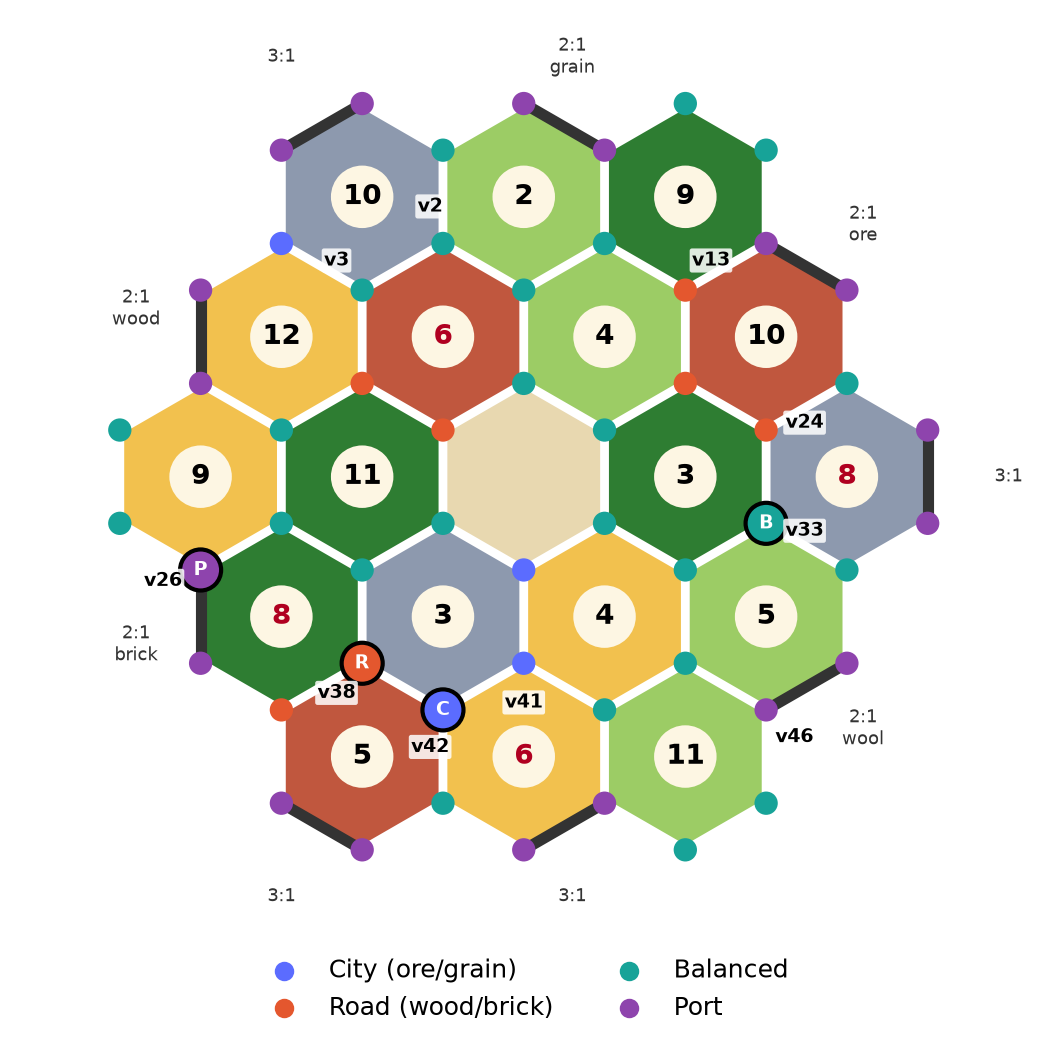
\includegraphics[width=0.6\textwidth]{board_categories.png}
\caption{Beginner board. Dots show each vertex's category (defined under ``Strategies'' below), and the large markers are each category's best spot.}\label{fig:board}
\end{figure}
\begin{figure}[htbp]\centering
\begin{minipage}[c]{0.47\textwidth}\centering\footnotesize\setlength{\tabcolsep}{4pt}
\topspots
\captionof{table}{Top two spots per category and their values $V$ at baseline ($\delta=\sigma=1$).}\label{tab:top}
\end{minipage}\hfill
\begin{minipage}[c]{0.49\textwidth}\centering
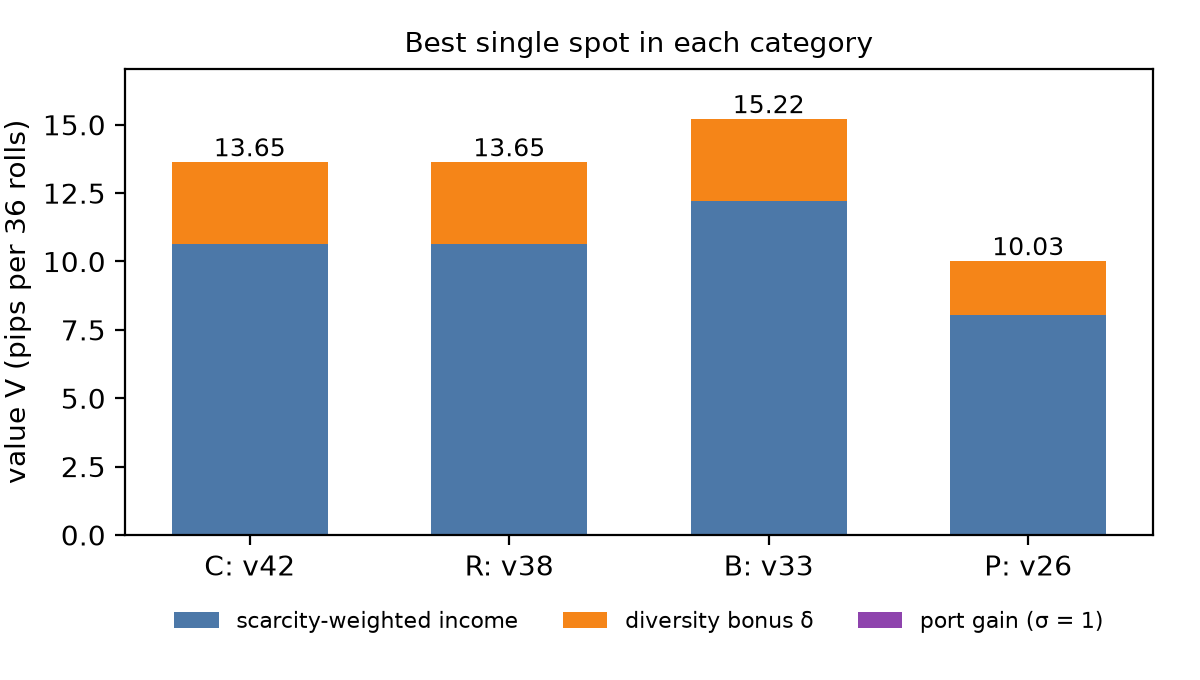
\includegraphics[width=\linewidth]{value_breakdown.png}
\captionof{figure}{What each category's best spot is worth. Even with $\sigma=1$, ports add little.}\label{fig:breakdown}
\end{minipage}
\end{figure}

\paragraph{Value of a hand.} We value a hand $S$ as
\begin{equation}\label{eq:V}
V(S) \;=\; \underbrace{\sum_r w_r\,\mathrm{prod}_S(r)}_{\text{income}} \;+\; \underbrace{\delta\cdot\#\{r:\mathrm{prod}_S(r)>0\}}_{\text{diversity}} \;+\; \underbrace{\sigma\sum_r \big(q_S(r)-\tfrac14\big)\,\mathrm{prod}_S(r)}_{\text{port gain}} .
\end{equation}
\begin{itemize}
\item \emph{Scarcity weights.} The board's supply $s_r$ of a resource is the total pips of its tiles: 13 for wood and grain, 12 for brick, and 10 for wool and ore. We value a resource in inverse proportion to its supply: $w_r=\bar s/s_r$, where $\bar s=11.6$ is the average supply. This gives $w=0.89$ for wood and grain, $0.97$ for brick, and $1.16$ for wool and ore.
\item \emph{Diversity.} Every building needs several resources, so each \emph{different} resource a player produces is worth a bonus $\delta$ (baseline $\delta=1$).
\item \emph{Ports.} The bank trades 4 of one card for 1 card of the trader's choice. A 3:1 port improves this to 3-for-1, and a 2:1 port for resource $r$ improves it to 2-for-1 \emph{for $r$ only}. Let $q_S(r)$ be the best rate (cards received per card given) open to $S$ for resource $r$: $\tfrac12$ with the 2:1 port for $r$, else $\tfrac13$ with any 3:1 port, else $\tfrac14$. Each card of $r$ traded then earns $q_S(r)-\tfrac14$ more than the bank would give. The parameter $\sigma$ is the share of income a player trades away. Our baseline $\sigma=1$ assumes \emph{every} card is traded, a generous upper bound on what a port is worth.
\end{itemize}
For example, $v_{46}$ sits on the 2:1 wool port and touches two wool tiles (6 pips), so its port gain is $(\tfrac12-\tfrac14)\cdot 6 = 1.5$. $v_{26}$ sits on the 2:1 \emph{brick} port but produces no brick, so on its own its port gain is $0$. A port's value depends on what its owner produces. In real games players trade far fewer cards, perhaps $\sigma\approx0.2$. We keep $\sigma=1$ as the baseline because it gives ports every advantage. If ports lose even then, they lose for any smaller $\sigma$, and Section~\ref{sec:robust} confirms that the draft is the same for every $\sigma\le1$.

\paragraph{Payoff.} P1 ends with hand $S_1$ and P2 with $S_2$. The payoffs are
\begin{equation}\label{eq:u}
u_1 = V(S_1)-V(S_2), \qquad u_2=-u_1 .
\end{equation}
\paragraph{Why the lead, and not the chance of winning?} What a player really wants is to win. Say P1's chance of winning is $f(u_1)$ for some increasing function $f$, so P2's is $1-f(u_1)$. We do not know $f$, but for our main results we do not need it. The draft has no randomness, so every way the draft can go ends in one definite lead $u_1$. Any increasing $f$ puts these endings in the same order: P1 prefers a larger lead and P2 a smaller one. Backward induction and the test for a pure Nash equilibrium only ever rely on which of two endings a player prefers. So they give the same answers whether the payoff is $u_1$ or $f(u_1)$.

\paragraph{Strategies.} Every vertex with production is assigned to one of four categories (Figure~\ref{fig:board}). \textbf{P} (Port) means the vertex touches a port. \textbf{C} (City) means ore and grain together make up at least half of its pips and it produces both. \textbf{R} (Road) is the same rule for wood and brick. \textbf{B} (Balanced) is everything else. Choosing a category means \emph{``take the still-legal vertex in that category that raises the mover's $V$ the most.''} Table~\ref{tab:top} lists the best spots in each category, and Figure~\ref{fig:breakdown} splits each value into the three terms of equation~\eqref{eq:V}: income, diversity and port gain.

\paragraph{Why categories?} We could instead let each move pick a specific vertex. We use categories for two reasons. First, they make strategies easy to interpret. A plan like ``split City then Road'' or ``take two Balanced spots'' says \emph{why} a spot is chosen, which a list of vertex numbers does not. Second, they make our analyses more computationally feasible. Finding every Nash equilibrium outcome and re-solving the draft across many parameter settings would be much larger tasks over individual vertices. We solve the exact vertex game only for a limited range of parameters, as a check. Section~\ref{sec:robust} shows that it gives the same answer there.

\paragraph{The game.} Four moves in the order P1, P2, P2, P1, each choosing a category with at least one legal vertex left. Both players see every earlier move, so this is a finite game with perfect information. It has 85 decision nodes and 254 end positions.


\section{Solving the Draft by Backward Induction}\label{sec:solve}
We solve from the end. P1's last move is easy: take the category that maximizes $u_1$. Next, P2's second move minimizes $u_1$, knowing how P1 will answer. Working backward in this way gives every node a \emph{value}: the lead P1 ends up with if both players play optimally from that node on. When a mover is exactly indifferent, we break the tie by the fixed order C, R, B, P. Section~\ref{sec:ne} shows that this choice does not matter.

Table~\ref{tab:reply} shows the top of the tree. Each row is an opening for P1, each column is P2's first reply, and each cell is P1's lead after the last two moves are played optimally. P2 will choose the reply that is worst for P1, the row minimum, so P1 opens with the row whose minimum is largest. This is a \emph{maximin} choice that can be checked by hand. Appendix~\ref{app:work} works out one cell of the table step by step and computes the hand values of Table~\ref{tab:hands}.

\begin{table}[h]\centering\small
\replytable
\caption{P1's lead (cards per 36 rolls) after P1's opening (row) and P2's first reply (column), with the last two moves played optimally. Bold: P2's best reply in each row. Boxed: P1's maximin opening.}\label{tab:reply}
\end{table}

\begin{result}\label{prop:spe}
The subgame-perfect equilibrium (SPE) path is $B\to C\to R\to B$. P1 first takes the best spot on the board, $v_{33}$ (wood~3, ore~8, wool~5). P2 then takes the best City spot $v_{42}$, followed by the Road spot $v_{13}$. Finally, P1 takes the brick/ore spot $v_3$. P1 leads by $u_1^*=0.83$ cards per 36 rolls (Table~\ref{tab:hands}, Figure~\ref{fig:spe}).
\end{result}
\begin{figure}[htbp]\centering
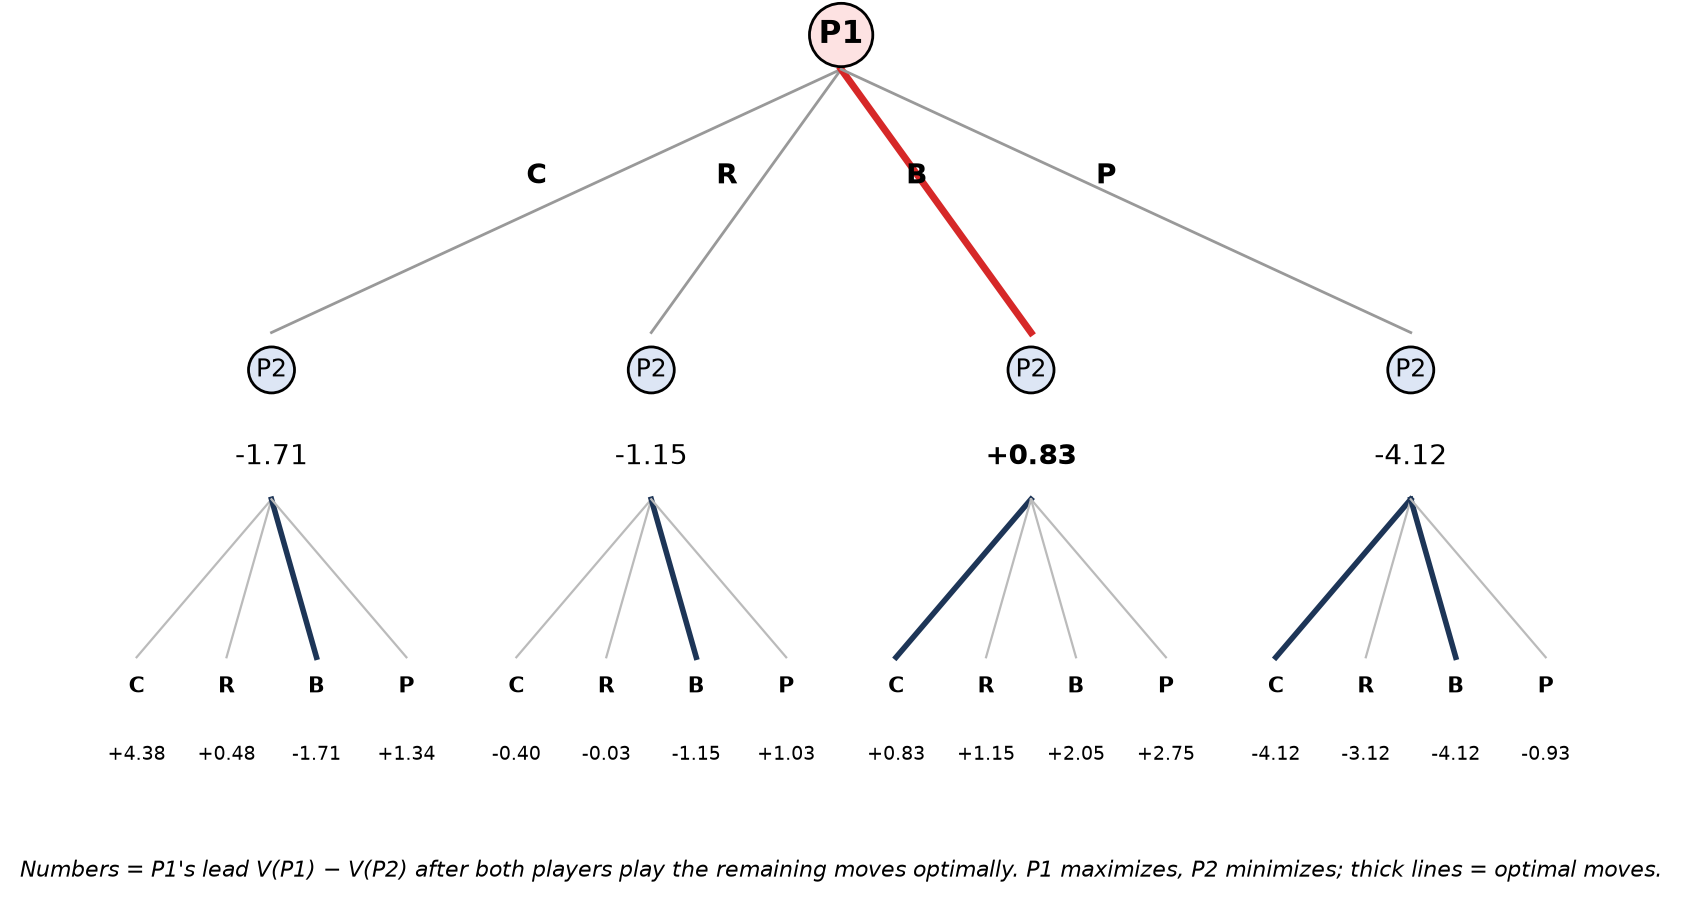
\includegraphics[width=0.53\textwidth]{sequential_tree.png}\hfill
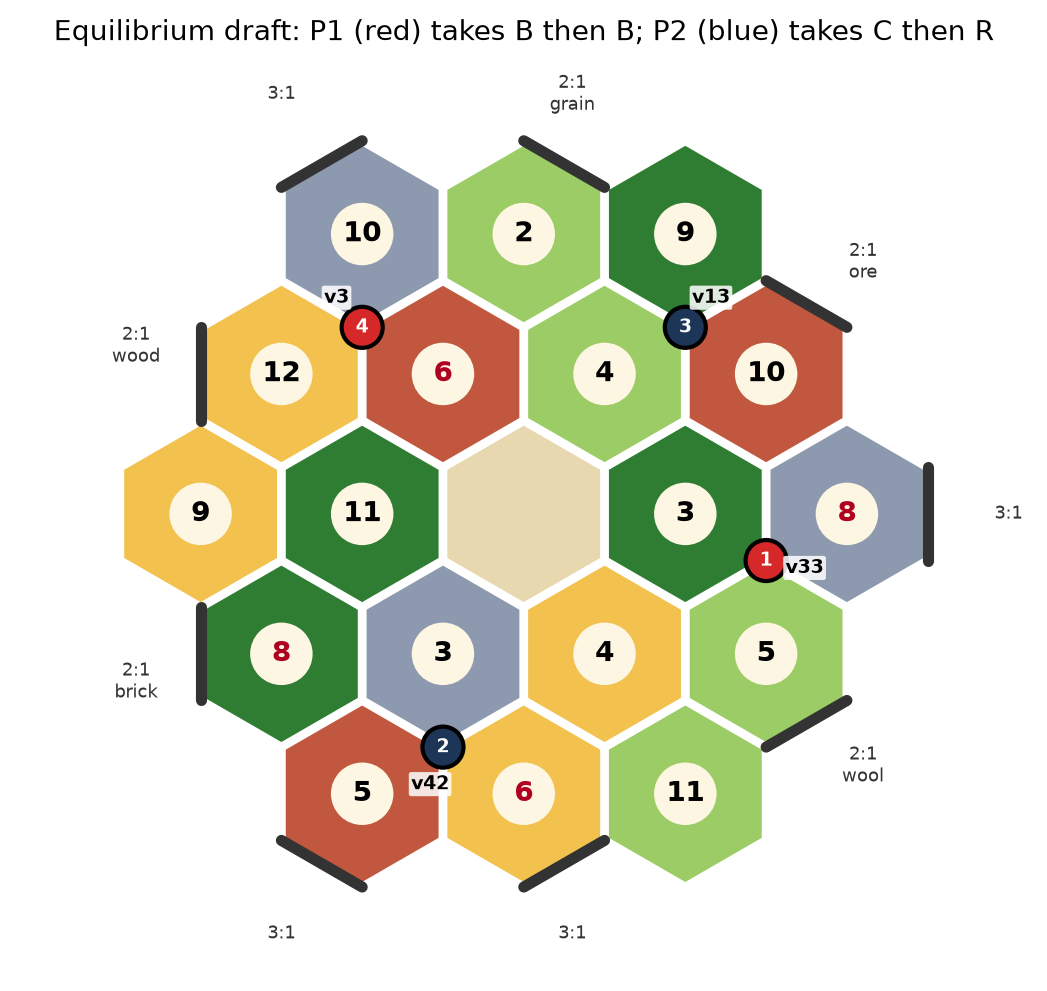
\includegraphics[width=0.44\textwidth]{sequential_board.png}
\caption{Left: top of the game tree with backward-induction values (P1's lead). Right: the equilibrium placements, numbered in draft order.}\label{fig:spe}
\end{figure}

\begin{table}[h]\centering\small
\handtable
\caption{The two players in the equilibrium. P1's lead is $26.43-25.60=0.83$.}\label{tab:hands}
\end{table}

Three things stand out. First, \textbf{nobody opens on a port}. A Port opening is P1's worst choice, at $-4.12$. Ports are only worth the cards they save in trade, and the spots next to them have poor production. Second, P2 answers the Balanced opening by \emph{splitting} the remaining good economies: the best ore/grain spot, then a wood/brick spot. Taking a second Balanced spot would leave P1 a lead of $2.05$, compared with $0.83$ after the City reply. Third, moving first is worth something: P1 ends ahead.


\section{All Nash Equilibria}\label{sec:ne}
In a sequential game, a \emph{strategy} is a complete plan. It says what the player would do at \emph{every} node where they move, including nodes that are never reached in actual play. For example, P2's strategy must say how P2 would reply to a Port opening, even though P1 never opens on a port. A \emph{Nash equilibrium} (NE) is a pair of strategies, one per player, such that neither player can gain by changing their own strategy while the other's stays the same. The \emph{outcome} of an NE is the sequence of moves that actually happens when both players follow it. Two NE can differ only at nodes that are never reached. Then they are different strategy pairs with the same outcome. So we answer two separate questions: which outcomes an NE can produce, and how many NE there are. (In the simultaneous games of a first course every move is actually played, so there are no unreached nodes and this distinction does not come up.) We use three classical facts~\cite{osborne}.

\begin{theorem}[Zermelo, Kuhn; von Neumann]\label{thm:minimax}
In a finite two-player zero-sum game with perfect information:
(i) backward induction yields a pure-strategy NE~\cite{zermelo,kuhn};
(ii) every NE, pure or mixed, gives P1 the same payoff, the \emph{value} $u_1^*$~\cite{vonneumann};
(iii) NE strategies are \emph{interchangeable}: if $(x,y)$ and $(x',y')$ are NE, then so are $(x,y')$ and $(x',y)$.
\end{theorem}
Part (ii) holds because in a zero-sum game an NE strategy is exactly a \emph{maximin} strategy: it guarantees its owner the most they can be sure of no matter what the opponent does. Both players' guarantees meet at one number, the value. So in our game \textbf{every Nash equilibrium gives $(u_1,u_2)=(0.83,-0.83)$}.

\paragraph{Every equilibrium outcome.} Which plays of the game can an NE produce? A play $z$ is an NE outcome exactly when no player on it can gain by deviating, even if the opponent then punishes as hard as possible. In a zero-sum game the hardest punishment is the opponent's optimal play, so a deviator receives the backward-induction value of the branch they deviate into. We applied this test to all 254 end positions. \textbf{Exactly one passes: $B\to C\to R\to B$.} So every NE produces the same draft. The NE themselves are not unique, because they can differ at nodes off this path, as we explain next.

\paragraph{Why there are infinitely many equilibria.} The NE test only asks whether a player gains by switching strategies. Changing a plan at a node that is never reached does not change what happens, so it changes nobody's payoff. A player's plan at an unreached node therefore does not have to be optimal. It only has to leave the opponent with no reason to go there. On the path itself every mover has one strictly best move (there are no ties), so no NE ever randomizes on the path. Off the path, there is a lot of freedom, in two ways.
\begin{enumerate}
\item \emph{Ties off the path.} At four nodes that are never reached in equilibrium, the mover is exactly indifferent (integer pips make exact ties possible). After $BB$ and $BP$, P2 is indifferent between C and R. After $PBB$, P1 is indifferent between C and R. After an opening $P$, P2 is indifferent between C and B. Any randomization at these nodes is part of an NE.
\item \emph{Plans that are not credible.} A move in a plan is \emph{credible} if the player would actually make it if that node were reached. Off the path, an NE plan can contain moves that are not credible. For example, a Port opening is very bad for P1: $-4.12$ against optimal play. So P2's plan can say ``after a Port opening, play a weak reply'' (or a random one). This weak reply helps P1, but even so, opening P is still worse for P1 than opening B: even P2's worst reply leaves P1 at only $-0.93$ (Table~\ref{tab:reply}), below $0.83$. P1 has no reason to deviate, so the pair is still an NE. But the plan is not credible: if P1 really did open P, P2 would not play the weak reply. P2 would play the optimal reply instead.
\end{enumerate}
Both kinds of freedom allow any amount of randomization, so there are \emph{infinitely many} Nash equilibria, most of them mixed. Theorem~\ref{thm:minimax} and our outcome test sum them up: all of them produce the draft $B\to C\to R\to B$ and the payoffs $(0.83,-0.83)$.

\section{Which Equilibrium Is Most Beneficial?}\label{sec:best}
In a non-zero-sum game, equilibria can differ in total welfare, and players may prefer different ones. In our zero-sum game \textbf{no equilibrium is better for either player than any other}: every one gives exactly $(0.83,-0.83)$. The total is always 0, so asking which equilibrium is ``best for both players'' has no payoff answer. Interchangeability (Theorem~\ref{thm:minimax}(iii)) also removes the coordination problem: each player can pick any equilibrium strategy independently and still reach an equilibrium.

We therefore select by \emph{credibility}. In most of the infinitely many NE, some player's plan contains a move they would not actually make if that node were reached, like the weak reply to a Port opening above. The \textbf{subgame-perfect equilibrium} (Result~\ref{prop:spe}) rules these out~\cite{selten}. It asks for an optimal move at every node, reached or not, so its plan stays optimal even after an opponent's mistake. A player who follows the SPE strategy never does worse than $0.83$ (P1) or $-0.83$ (P2), and gains whenever the opponent errs. The four off-path ties mean the SPE strategy is not literally unique, but all its versions are equivalent and play the same draft. This is the equilibrium we recommend: \textbf{open on the best Balanced spot; as P2, split City then Road.}

\paragraph{Fairness of the snake order.} The equilibrium favors P1. The snake order is designed to offset this by giving P2 two picks in a row. If the order were alternating (P1, P2, P1, P2), the value would be $1.15$ (draft $B\to R\to B\to B$), compared with $0.83$ under the snake. So the snake order removes about 27\% of P1's advantage, but not all of it. We solved the alternating game by the same backward induction, with only the order of movers changed.

\section{Robustness}\label{sec:robust}
\paragraph{Categories versus individual spots.} Choosing among four categories is a simplification. We therefore also solved the \emph{exact} game in which each move picks a specific vertex. P1 picks one vertex, P2 picks two vertices in a row (a joint choice), and P1 answers with the best remaining vertex. The exact game has the same value, $0.83$, and the same four spots. Over the 48 parameter settings we checked, the two games agree whenever the scarcity weights are on (24 of 24) and whenever $\sigma\le1$. All 7 disagreements have scarcity weights off and $\sigma\ge2$.

\paragraph{Parameters.} We re-solved the draft on a grid of 442 settings: $\delta\in[0,3]$, $\sigma\in[0,4]$ (in steps of $0.25$), with scarcity weights on and off (Figure~\ref{fig:sens}).
\begin{itemize}
\item With scarcity weights on, the draft is $B\to C\to R\to B$ for \textbf{every} $\delta\in[0,3]$ and \textbf{every} $\sigma\le1$, that is, for every port valuation up to the ``trade everything'' bound. The equilibrium outcome is unique at 92\% of these settings.
\item Ports enter the equilibrium only when $\sigma\ge1.25$ (for $\delta\le0.25$). The threshold rises to $\sigma\ge1.75$ at the baseline $\delta=1$ and to $\sigma\ge2.25$ for every $\delta\ge1.5$. A port would have to be worth more than its entire trading benefit, which no amount of trading can deliver.
\item Without scarcity weights, all resources count equally and P1 opens on \textbf{City} instead ($C\to B\to B\to R$ in most settings with $\sigma\le1$). The weights matter because the Balanced spot $v_{33}$ is rich in the scarce resources ore and wool.
\item P1 is ahead in 83\% of all settings. The snake order is never worse for P2 than alternating order. It is strictly better in 47\% of settings (62\% when $\sigma\le1$), and in the rest the two orders give the same value.
\end{itemize}

\begin{figure}[htbp]\centering
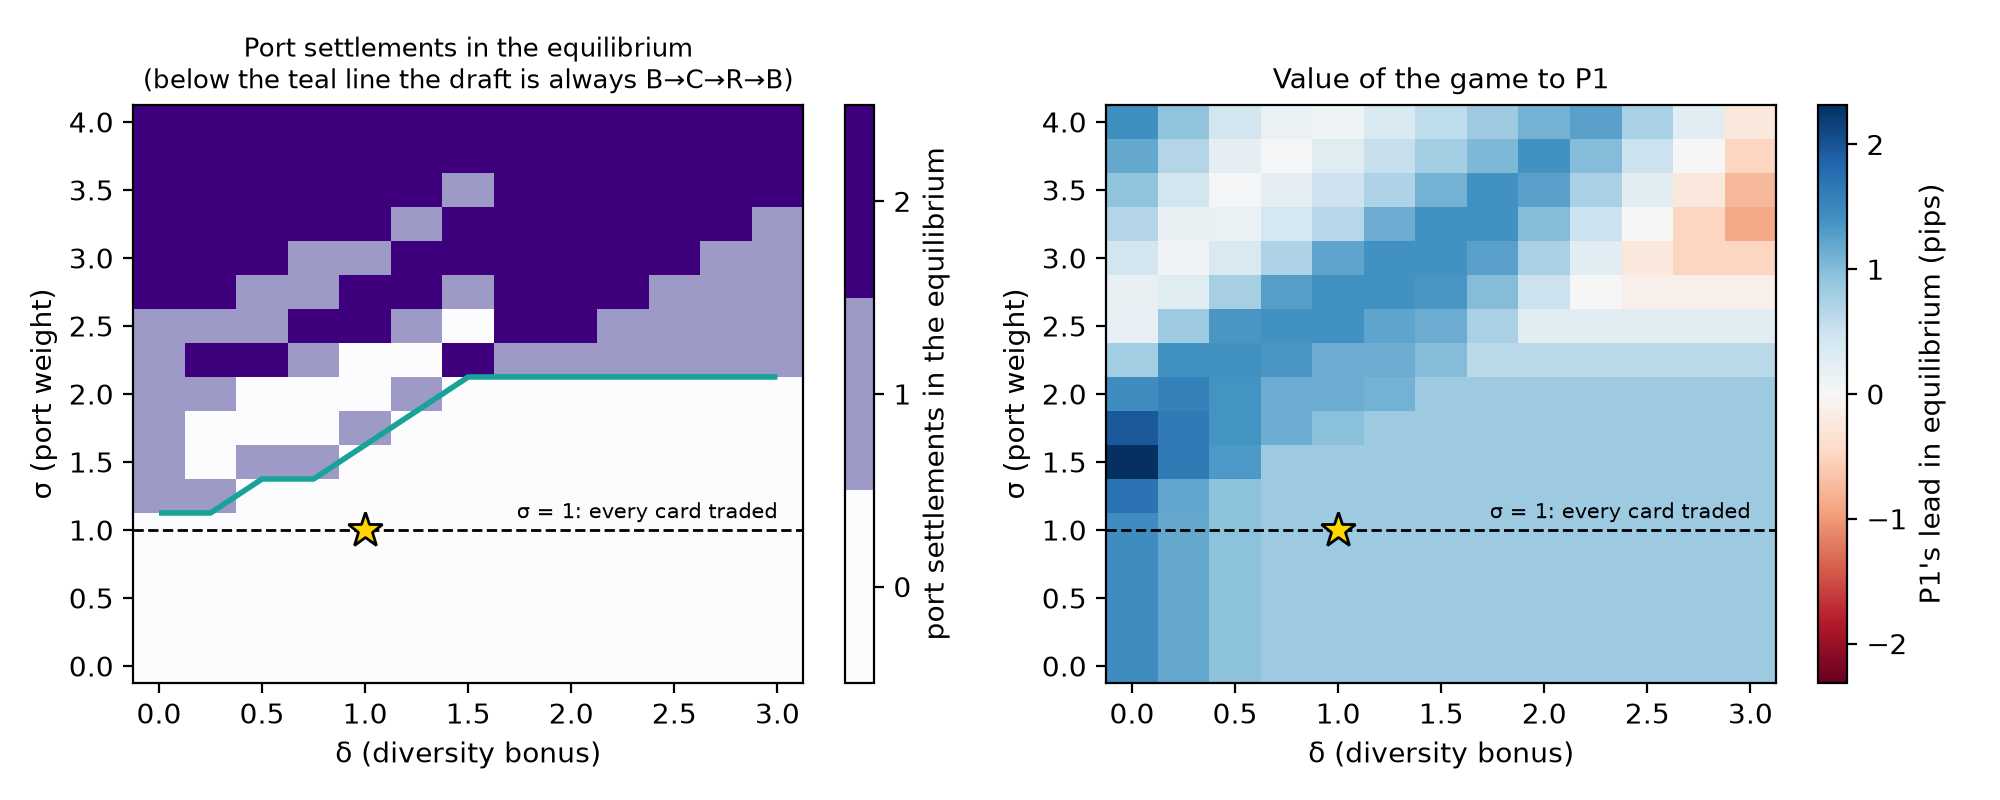
\includegraphics[width=0.98\textwidth]{sensitivity.png}
\caption{Robustness with scarcity weights on; the star marks the baseline. Left: the number of port settlements in the equilibrium draft. Below the teal line the draft is always $B\to C\to R\to B$. Right: the value of the game to P1.}\label{fig:sens}
\end{figure}

\section{Discussion and Limitations}\label{sec:disc}
Our value function counts income, not victory points. It ignores the robber, development cards, and the races for the longest road and the largest army. A real player may also value wood and brick beyond their pips, because they build the roads and settlements needed to expand early. Our payoff also assumes that a player's chance of winning depends only on their \emph{lead}. If, for example, ore helped a player win more than its income suggests, the chance of winning would depend on the mix of resources and not only on the lead. Port values are an upper bound ($\sigma=1$), and ports still lose, so that conclusion is conservative. On random boards the answer would change, but the method (backward induction, the maximin table, the outcome test) carries over.

A non-zero-sum version (for example, payoff = own income) could have several equilibria with different payoffs, and the players would then have to agree on which one to play. Real two-player \emph{Catan} has no such problem: a move that raises both players' income equally does not change either player's chance of winning.

\section{Conclusion}
As a two-player zero-sum game on the beginner board, the \emph{Catan} opening has a unique equilibrium outcome: \textbf{P1 takes the best Balanced spot, P2 answers with City then Road, and P1 finishes with another Balanced spot}, ahead by $0.83$ cards per 36 rolls. There are infinitely many Nash equilibria, but by the minimax theorem they are payoff-equivalent and interchangeable, so the most beneficial one is the credible one: the subgame-perfect equilibrium. Valued by what they actually save in trades, ports are not worth opening on. The snake order reduces the first mover's advantage by about a quarter.

\paragraph{Code and data.} All code, data and figures are at \url{https://github.com/JadonJZhu/catan-opening-game-theory}. One script (\texttt{analysis/run\_all.py}) reproduces every number, table and figure in this paper. An interactive web app at \url{https://jadonjzhu.github.io/catan-opening-game-theory/webapp/} lets the reader change $\delta$, $\sigma$ and the scarcity weights and re-solve the draft.

\paragraph{Use of AI.}
We used an AI assistant (Claude) to help design the model, write the analysis code and figures, and draft text. Every number in this paper is produced by our code, and we checked the backward-induction values in Table~\ref{tab:reply} and the hand values in Table~\ref{tab:hands} by hand.

\begin{thebibliography}{9}\footnotesize\setlength{\itemsep}{0pt}
\bibitem{zermelo} E.~Zermelo. \"Uber eine Anwendung der Mengenlehre auf die Theorie des Schachspiels. \emph{Proc.\ 5th ICM}, 2:501--504, 1913.
\bibitem{kuhn} H.~W.~Kuhn. Extensive games and the problem of information. \emph{Ann.\ Math.\ Studies} 28:193--216, 1953.
\bibitem{vonneumann} J.~von Neumann. Zur Theorie der Gesellschaftsspiele. \emph{Mathematische Annalen}, 100:295--320, 1928.
\bibitem{selten} R.~Selten. Reexamination of the perfectness concept for equilibrium points in extensive games. \emph{Int.\ J.\ Game Theory}, 4:25--55, 1975.
\bibitem{osborne} M.~J.~Osborne. \emph{An Introduction to Game Theory}. Oxford University Press, 2004.
\bibitem{hotelling} H.~Hotelling. Stability in competition. \emph{The Economic Journal}, 39(153):41--57, 1929.
\bibitem{catan} K.~Teuber. \emph{Catan} base game rules and almanac (beginner set-up). Catan GmbH.
\end{thebibliography}
\appendix
\section{Worked Computations}\label{app:work}
\paragraph{Hand values.} We compute $V$ for the two equilibrium hands in Table~\ref{tab:hands}. The weights are $w=11.6/13\approx0.892$ for wood and grain, $11.6/12\approx0.967$ for brick, and $11.6/10=1.160$ for wool and ore. P1 holds $v_{33}$ and $v_3$, which together produce wood 2, brick 5, wool 4, grain 1 and ore 8 pips. So
\[
\text{income}_1 = 0.892\cdot2 + 0.967\cdot5 + 1.160\cdot4 + 0.892\cdot1 + 1.160\cdot8 \approx 21.43 .
\]
P1 produces all 5 resources, so the diversity term is $\delta\cdot5=5$. Neither spot is on a port, so $q(r)=\tfrac14$ for every $r$ and the port gain is $0$. Thus $V(S_1)\approx26.43$. P2 holds $v_{42}$ and $v_{13}$, producing wood 4, brick 7, wool 3, grain 5 and ore 2:
\[
\text{income}_2 = 0.892\cdot4 + 0.967\cdot7 + 1.160\cdot3 + 0.892\cdot5 + 1.160\cdot2 \approx 20.60 ,
\]
plus 5 for diversity and $0$ for ports, so $V(S_2)\approx25.60$ and $u_1\approx0.83$.

\paragraph{One branch of backward induction.} We compute the cell ``P1 opens B, P2 replies C'' of Table~\ref{tab:reply}. After $\workedprefix$, P2 moves (third pick) and then P1 moves (last pick). Table~\ref{tab:worked} lists P1's final lead for each pair of choices. Each lead is $V(S_1)-V(S_2)$ for the resulting hands, computed as above.
\begin{table}[h]\centering\small
\workedtable
\caption{After $\workedprefix$: P1's lead for each third pick by P2 (row) and last pick by P1 (column). Bold: P1's best last pick. Boxed: P2's best third pick.}\label{tab:worked}
\end{table}

\noindent We solve it from the end. In each row, P1 makes the last move and takes the largest entry (bold), which is the row maximum. P2 moves before that and knows how P1 will answer, so P2 picks the row with the \emph{smallest} maximum. That is row R, with value $0.83$. This is the B/C cell of Table~\ref{tab:reply}. The other cells come from the same two steps, and the root then follows from the row minima of Table~\ref{tab:reply}.

\end{document}
